% =============================================================================
%  slides.tex: 15 minute overview of the RISC-V vector (RVV) work in
%  pystencils and waLBerla, for listeners who know software but not this
%  project. Build with ./build.sh (output: build/slides.pdf).
%
%  Sources of every number: docs/manual/reports/r02 (making RVV work) and
%  docs/manual/reports/r03 (making it fast), which cite the raw board logs in
%  docs/notes3/board-logs/. The results slides and the prefetch and in-place
%  takeaways use one session with every build on 1, 4 and 8 cores (GCC 14, 64^3
%  cells per core, best of 3 runs of 200 steps): docs/notes3/board-logs/presentation3/,
%  written by scripts/presentation3/all.sh. The backup table "one step at a
%  time" keeps the history from r03 "run B" and "run C".
%
%  Writing rules: plain English, short sentences, no em/en dashes as
%  punctuation, every name explained where it first appears and again in the
%  glossary at the end.
% =============================================================================
\documentclass[aspectratio=169,10pt,t]{beamer}

\usepackage[T1]{fontenc}
\usepackage[utf8]{inputenc}
\usepackage[sfdefault,lining]{FiraSans}
\usepackage[varqu]{inconsolata}
\usefonttheme{professionalfonts}
\usepackage{amsmath,amssymb}
\usepackage{booktabs,array,tabularx}
\usepackage{pifont}
\usepackage{appendixnumberbeamer}

\usepackage{tikz}
\usetikzlibrary{positioning,arrows.meta,calc,fit,backgrounds,decorations.pathreplacing,patterns}
\usepackage{pgfplots}
\pgfplotsset{compat=1.18}

% ---- Colours (the same as in docs/manual, so slides and reports match) --------
\definecolor{psblue}{HTML}{1F5FA8}
\definecolor{psteal}{HTML}{127A72}
\definecolor{psorange}{HTML}{C8641A}
\definecolor{psred}{HTML}{B3261E}
\definecolor{psgray}{HTML}{5F6368}
\definecolor{codebg}{HTML}{F6F8FA}
\definecolor{psviolet}{HTML}{7A3E9D}   % generated code (build-run figure)
\newif\ifbrmarkers                       % markers in figures/build-run.tex
%   Meaning of the colours in every figure:
%   teal = added and measured, orange = in the code but not measured yet,
%   red = tried and dropped (or: what was wrong before), blue = facts about the hardware.

% ---- Beamer look ------------------------------------------------------------------
\setbeamersize{text margin left=8mm,text margin right=8mm}
\setbeamertemplate{navigation symbols}{}
\setbeamercolor{normal text}{fg=black!88}
\setbeamercolor{structure}{fg=psblue}
\setbeamercolor{frametitle}{fg=psblue!80!black}
\setbeamerfont{frametitle}{size=\large,series=\bfseries}
\setbeamercolor{itemize item}{fg=psblue}
\setbeamercolor{itemize subitem}{fg=psgray}
\setbeamertemplate{itemize item}{\raisebox{0.15ex}{\small$\bullet$}}
\setbeamertemplate{itemize subitem}{\raisebox{0.1ex}{\scriptsize$\circ$}}
\setlength{\leftmargini}{1.1em}
\setlength{\leftmarginii}{1.1em}
\setbeamercolor{takeaway}{bg=psblue!8,fg=black!88}

\setbeamertemplate{frametitle}{%
  \nointerlineskip\vskip3mm
  \hbox to \textwidth{%
    \usebeamerfont{frametitle}\usebeamercolor[fg]{frametitle}\insertframetitle\hfil
    {\usebeamerfont{footline}\scriptsize\color{psgray}\insertsectionhead}}%
  \vskip1.5mm
  {\color{psblue!40}\hrule height 0.5pt}%
  \vskip1mm}

\setbeamertemplate{footline}{%
  \hbox to \paperwidth{\hspace*{8mm}{\color{psgray}\tiny RISC-V vectors in pystencils and waLBerla}%
    \hfil{\color{psgray}\tiny\insertframenumber\,/\,\inserttotalframenumber}\hspace*{8mm}}%
  \vskip2.5mm}

% ---- Macros -------------------------------------------------------------------------
\newcommand{\presenter}{Saleh}            % edit: name on the title slide
\newcommand{\sx}[1]{#1\ensuremath{\times}} % a speedup factor, e.g. \sx{5.24}
\newcommand{\term}[1]{\textcolor{psblue!85!black}{\textbf{#1}}} % a name, defined right here
\newcommand{\code}[1]{\texttt{#1}}
\newcommand{\yes}{\textcolor{psteal}{\ding{51}}}
\newcommand{\no}{\textcolor{psgray!70}{$\cdot$}}
\newcommand{\tagdot}[1]{\tikz[baseline=-0.6ex]\fill[#1] (0,0) circle (0.9mm);} % colour dot
%   \todo{text}: a measurement or fact that is still missing. Shown in red; build with
%   ./build.sh final to hide all of them (it defines \hidetodos). ./build.sh lists them.
\newif\ifshowtodos \showtodostrue
\ifdefined\hidetodos \showtodosfalse \fi
\newcommand{\todo}[1]{\ifshowtodos{\scriptsize\textcolor{psred}{\textbf{[TODO: #1]}}}\fi}
%   \takeaway{text}: the one sentence to remember, at the bottom of a slide
\newcommand{\takeaway}[1]{\par\vfill
  \begin{beamercolorbox}[wd=\textwidth,sep=4pt,rounded=true]{takeaway}
    \small #1
  \end{beamercolorbox}}

% ---- TikZ styles shared by the figures ------------------------------------------------
\tikzset{
  box/.style={draw=psgray!80,fill=white,rounded corners=2pt,align=center,
    font=\footnotesize,inner sep=3pt,minimum height=7mm},
  added/.style={box,fill=psteal!12,draw=psteal!90!black,line width=0.6pt},
  pending/.style={box,fill=psorange!12,draw=psorange!90!black,line width=0.6pt},
  wrong/.style={box,fill=psred!7,draw=psred!80!black,line width=0.6pt},
  info/.style={box,fill=psblue!7,draw=psblue!70!black},
  quiet/.style={box,fill=psgray!8,draw=psgray!60,text=psgray!90!black},
  arr/.style={-{Stealth[length=2mm]},semithick,draw=psgray!90!black},
  lbl/.style={font=\scriptsize,text=psgray!90!black,align=center},
  codebox/.style={box,fill=codebg,font=\ttfamily\scriptsize,align=left,inner sep=4pt},
}

\title{Vector instructions for a generated fluid simulation on RISC-V}
\subtitle{What we added to pystencils and waLBerla, how it works,\\and what it gives on one SpacemiT X60 core}
\author{\presenter}
\date{November 2026}

\begin{document}

% =============================================================================
\begin{frame}[plain]
  \begin{tikzpicture}[remember picture,overlay]
    % a strip of 8 "vector lanes" along the top edge
    \foreach \k in {0,...,7}
      \fill[psblue!\the\numexpr 25+8*\k\relax] ([xshift=\k*20mm]current page.north west) rectangle ++(19.6mm,-3mm);
    \node[anchor=north west,text width=136mm,align=left,inner sep=0pt,
          execute at begin node={\hyphenpenalty=10000\exhyphenpenalty=10000}]
      at ([xshift=12mm,yshift=-22mm]current page.north west) {%
      {\LARGE\bfseries\color{psblue!80!black}\inserttitle\par}
      \vspace{5mm}
      {\large\color{black!75}\insertsubtitle\par}
      \vspace{14mm}
      {\normalsize\insertauthor\par}
      \vspace{1mm}
      {\normalsize\color{psgray}\insertdate\par}};
  \end{tikzpicture}
\end{frame}

% =============================================================================
% =============================================================================
\section{Background}

\begin{frame}{The benchmark: a fluid in a periodic box}
  \vspace{1mm}
  \begin{columns}[T,onlytextwidth]
    \column{0.40\textwidth}
    \centering% Slide "The benchmark": the flow of waLBerla's DoubleShearLayer example, as the benchmark
% SweepgenLbmCPU sets it up (report r03, "The benchmark application"): a fully periodic box;
% u_x = u0 tanh(kappa (y - 1/4)) for y <= 1/2 and u0 tanh(kappa (3/4 - y)) above, so the middle
% band moves right, the outer bands left, with two shear layers at y = 1/4 and 3/4; a small
% sine perturbation u_y = delta u0 sin(2 pi (x + 1/4)) makes them roll up. Cross-section, 2D.
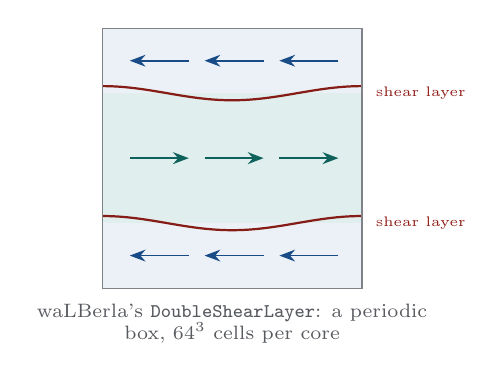
\begin{tikzpicture}
  \def\L{3.3}
  \fill[psblue!9]  (0,0) rectangle (\L,\L/4);
  \fill[psteal!13] (0,\L/4) rectangle (\L,3*\L/4);
  \fill[psblue!9]  (0,3*\L/4) rectangle (\L,\L);
  \foreach \yy in {0.25,0.75}
    \draw[psred!75!black,thick,smooth,samples=40,domain=0:\L]
      plot (\x,{\yy*\L+0.09*sin(360*(\x/\L+0.25))});
  \draw[psgray!80] (0,0) rectangle (\L,\L);
  \foreach \x in {0.35,1.3,2.25} {
    \draw[arr,psteal!80!black,thick] (\x,\L/2) -- ++(0.75,0);
    \draw[arr,psblue!80!black] (\x+0.75,\L/8) -- ++(-0.75,0);
    \draw[arr,psblue!80!black] (\x+0.75,7*\L/8) -- ++(-0.75,0);
  }
  \node[font=\tiny,text=psred!80!black,anchor=west] at (\L+0.05,3*\L/4) {shear layer};
  \node[font=\tiny,text=psred!80!black,anchor=west] at (\L+0.05,\L/4) {shear layer};
  \node[lbl,anchor=north] at (\L/2,-0.08) {waLBerla's \code{DoubleShearLayer}: a periodic\\box, $64^3$ cells per core};
\end{tikzpicture}

    \column{0.57\textwidth}
    \centering\resizebox{!}{4.1cm}{% Slide 3: the two halves of an LBM time step, drawn in 2D (9 directions) for readability.
% The real model, D3Q19, is 3D with 19 directions.
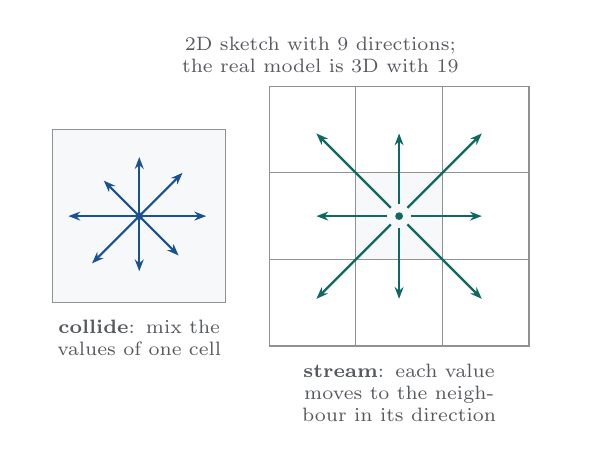
\begin{tikzpicture}[
    pdf/.style={-{Stealth[length=1.5mm]},thick,draw=psblue!85!black},
    mv/.style={-{Stealth[length=1.5mm]},thick,draw=psteal!85!black}]
  % ---- collide: one cell, one value per direction (arrow length = value)
  \draw[psgray!70,fill=codebg] (0,0.55) rectangle (2.2,2.75);
  \coordinate (c) at (1.1,1.65);
  \foreach \dx/\dy/\l in {1/0/0.85, 1/1/0.55, 0/1/0.75, -1/1/0.45, -1/0/0.9, -1/-1/0.6, 0/-1/0.7, 1/-1/0.5} {
    \draw[pdf] (c) -- ++({\dx*\l},{\dy*\l});
  }
  \fill[psblue!85!black] (c) circle (1.4pt);
  \node[lbl,anchor=north,text width=26mm] at (1.1,0.45) {\textbf{collide}: mix the values of one cell};

  % ---- stream: each value moves to the neighbour in its direction
  \begin{scope}[xshift=2.75cm]
    \foreach \i in {0,1,2} \foreach \j in {0,1,2}
      \draw[psgray!70,fill=white] (\i*1.1,\j*1.1) rectangle ++(1.1,1.1);
    \fill[codebg] (1.1,1.1) rectangle ++(1.1,1.1);
    \draw[psgray!70] (1.1,1.1) rectangle ++(1.1,1.1);
    \coordinate (s) at (1.65,1.65);
    \foreach \dx/\dy in {1/0, 1/1, 0/1, -1/1, -1/0, -1/-1, 0/-1, 1/-1}
      \draw[mv,shorten <=1.5mm] (s) -- ++({\dx*1.05},{\dy*1.05});
    \fill[psteal!85!black] (s) circle (1.4pt);
    \node[lbl,anchor=north,text width=33mm] at (1.65,-0.1) {\textbf{stream}: each value moves to the neighbour in its direction};
  \end{scope}
  \node[lbl,anchor=south,text width=60mm] at (3.4,3.35) {2D sketch with 9 directions; the real model is 3D with 19};
\end{tikzpicture}
}
  \end{columns}

  \vspace{3mm}
  {\small \term{waLBerla}: C++ fluid simulation framework. \term{Lattice Boltzmann method}, 19
  numbers per cell (\term{D3Q19}). 200 time steps; speed in \term{MLUP/s}, million cell updates per
  second.\par}
  \takeaway{Per cell and time step: 19 loads, about 200 operations, 19 stores.}
\end{frame}

% -----------------------------------------------------------------------------
\begin{frame}{The hardware, and how the work is split}
  \vspace{3mm}
  \centering% Slide "The hardware, and how the work is split": the SpacemiT K1 on the Banana Pi BPI-F3
% (report r03, table "test system"): 8 X60 cores at 1.6 GHz in two clusters of 4; L1D 32 KiB per
% core, L2 512 KiB per cluster, no L3; 4 GB memory, about 357 cycles per DRAM miss (pointer chase,
% huge pages). The benchmark runs one MPI process with one 64^3 block per core.
% Right: one X60 core's 256-bit vector register as 8 f32 or 4 f64 lanes.
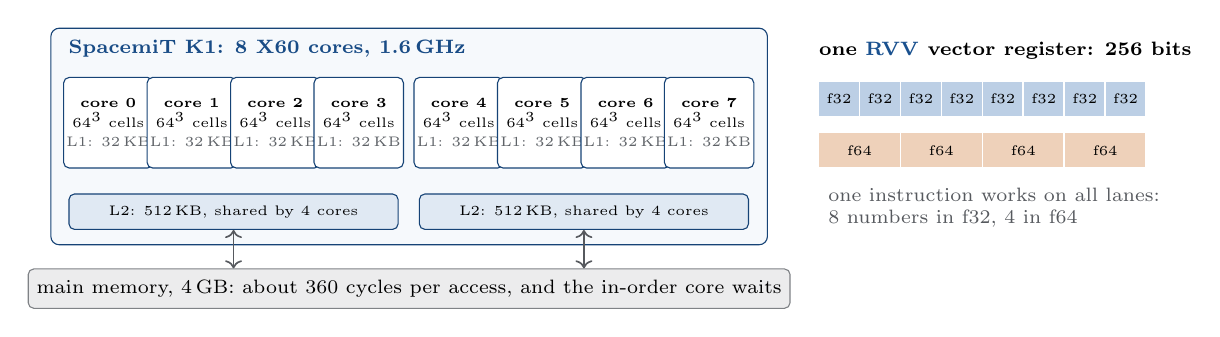
\begin{tikzpicture}[
    core/.style={box,minimum width=0.98cm,minimum height=1.15cm,fill=white,draw=psblue!70!black,
      font=\tiny,align=center,inner sep=1pt},
    l2/.style={box,fill=psblue!14,draw=psblue!70!black,font=\tiny,minimum height=4.5mm,inner sep=1pt},
    ln/.style={draw=white,line width=0.6pt,minimum height=4.5mm,inner sep=0pt,font=\tiny}]
  % ---- the chip -------------------------------------------------------------------
  \draw[psblue!70!black,fill=psblue!4,rounded corners=3pt] (0,0) rectangle (9.1,2.75);
  \node[anchor=north west,font=\scriptsize\bfseries,text=psblue!80!black] at (0.1,2.72)
    {SpacemiT K1: 8 X60 cores, 1.6\,GHz};
  \foreach \c/\xo in {0/0.2,1/4.65} {
    \foreach \k in {0,...,3} {
      \pgfmathtruncatemacro{\n}{4*\c+\k}
      \node[core] at (\xo+0.53+\k*1.06,1.55) {\textbf{core \n}\\[1pt]$64^3$ cells\\[1pt]{\color{psgray}L1: 32\,KB}};
    }
    \node[l2,minimum width=4.18cm] (l\c) at (\xo+2.12,0.42) {L2: 512\,KB, shared by 4 cores};
  }
  % ---- main memory -------------------------------------------------------------------
  \node[box,fill=psgray!12,minimum width=9.1cm,minimum height=5mm,font=\scriptsize,anchor=north]
    (mem) at (4.55,-0.3) {main memory, 4\,GB: about 360 cycles per access, and the in-order core waits};
  \foreach \c in {0,1} \draw[<->,semithick,psgray!90!black] (l\c.south) -- (l\c.south |- mem.north);

  % ---- one core's vector register --------------------------------------------------
  \begin{scope}[shift={(9.75,0.25)}]
    \def\w{0.52}
    \node[font=\scriptsize\bfseries,anchor=south west,inner sep=0pt] at (0,2.1) {one \term{RVV} vector register: 256 bits};
    \foreach \k in {0,...,7}
      \node[ln,fill=psblue!30,minimum width=\w cm] at (\k*\w+\w/2,1.6) {f32};
    \foreach \k in {0,...,3}
      \node[ln,fill=psorange!30,minimum width=2*\w cm] at (\k*2*\w+\w,0.95) {f64};
    \node[lbl,anchor=north west,align=left] at (0,0.6)
      {one instruction works on all lanes:\\8 numbers in f32, 4 in f64};
  \end{scope}
\end{tikzpicture}


  \vspace{4mm}
  \raggedright
  {\small One \term{MPI} process and one block per core. After every step, neighbouring blocks swap
  their border cells (\term{halo exchange}).\par}
  \takeaway{One 256-bit operation per cycle: at best \sx{8} (f32) and \sx{4} (f64). These are our
    goals.}
\end{frame}

% -----------------------------------------------------------------------------
\begin{frame}{From source code to a running simulation}
  \vspace{1mm}
  \centering% From source to a running simulation (report r02, chapter "Code Generation" and its figure
% build-flow.tex). CMake configures; during "make", CMake runs the Python generator scripts
% (sweepgen sets jit = no_jit: generate only), then compiles the generated C++ together with
% the hand-written waLBerla core. The executable runs without Python. Everything ran on the
% board. Violet = generated code. Each column is one step; the small arrows between the
% headers carry the results from step to step (no wires across columns).
%
% With \brmarkerstrue (slide "Where each change lives") numbered markers show what we changed:
% blue = part 1, teal = part 2 (10 to 12: the last three changes, see the open-work slide).
% The markers sit on the nodes a2, g0, g2, g3, i1, i2 and cc.
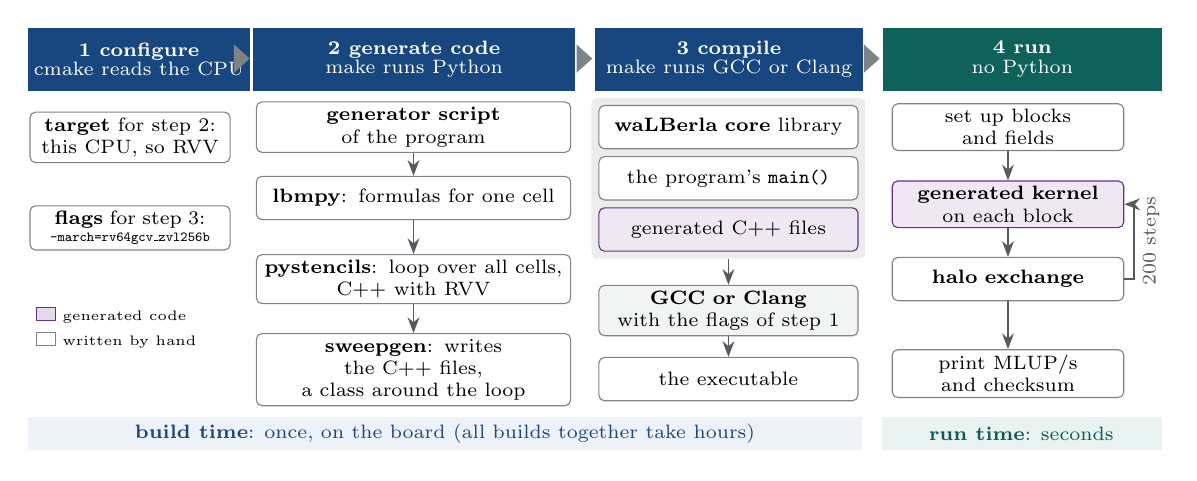
\begin{tikzpicture}[
    hdr/.style={font=\scriptsize\bfseries,text=white,align=center,inner sep=2pt,
      minimum height=8mm,anchor=north west},
    b/.style={box,font=\scriptsize,minimum height=5.5mm,inner sep=2pt,
      execute at begin node={\hyphenpenalty=10000\exhyphenpenalty=10000}},
    gen/.style={b,fill=psviolet!12,draw=psviolet!80!black},
    hdrarr/.style={fill=psgray!80},
    mk/.style={circle,text=white,font=\tiny\bfseries,inner sep=0pt,minimum size=3.7mm}]
  \ifbrmarkers\tikzset{mkl/.style={align=left}}\else\tikzset{mkl/.style={}}\fi
  % ---- column headers, with arrows from step to step --------------------------------
  \node[hdr,fill=psblue!75!black,minimum width=2.6cm] at (0,0)
    {1 configure\\[-1pt]{\mdseries cmake reads the CPU}};
  \node[hdr,fill=psblue!75!black,minimum width=4.1cm] at (2.85,0)
    {2 generate code\\[-1pt]{\mdseries make runs Python}};
  \node[hdr,fill=psblue!75!black,minimum width=3.4cm] at (7.2,0)
    {3 compile\\[-1pt]{\mdseries make runs GCC or Clang}};
  \node[hdr,fill=psteal!80!black,minimum width=3.55cm] at (10.85,0)
    {4 run\\[-1pt]{\mdseries no Python}};
  \foreach \x in {2.62,6.97,10.62}
    \fill[hdrarr] (\x,-0.22) -- ++(0.2,-0.18) -- ++(-0.2,-0.18) -- cycle;

  % ---- 1 configure: two settings for the later steps --------------------------------
  \node[b,text width=2.4cm] (a3) at (1.3,-1.4) {\textbf{target} for step 2:\\this CPU, so RVV};
  \node[b,text width=2.4cm,font=\tiny] (a2) at (1.3,-2.55)
    {{\scriptsize\textbf{flags} for step 3:}\\\code{-march=rv64gcv\_zvl256b}};
  \node[anchor=north west,font=\tiny,align=left,inner sep=0pt] at (0.1,-3.55)
    {\tikz\fill[psviolet!20,draw=psviolet!80!black] (0,0) rectangle (2.4mm,1.6mm);\ generated code\\[3pt]
     \tikz\draw[psgray!80] (0,0) rectangle (2.4mm,1.6mm);\ written by hand};

  % ---- 2 generate: the Python tool chain ---------------------------------------------
  \node[b,text width=3.85cm] (g0) at (4.9,-1.27) {\textbf{generator script} of the program};
  \node[b,text width=3.85cm] (g1) at (4.9,-2.17) {\textbf{lbmpy}: formulas for one cell};
  \node[b,text width=3.85cm] (g2) at (4.9,-3.2) {\textbf{pystencils}: loop over all cells,\\C++ with RVV};
  \node[b,text width=3.85cm] (g3) at (4.9,-4.35) {\textbf{sweepgen}: writes the C++ files,\\a class around the loop};
  \foreach \u/\v in {g0/g1,g1/g2,g2/g3} \draw[arr] (\u) -- (\v);

  % ---- 3 compile: hand-written and generated C++ together ----------------------------
  \node[b,mkl,text width=3.15cm] (i1) at (8.9,-1.27) {\textbf{waLBerla core} library};
  \node[b,mkl,text width=3.15cm] (i2) at (8.9,-1.92) {the program's \code{main()}};
  \node[gen,text width=3.15cm] (i0) at (8.9,-2.57) {generated C++ files};
  \begin{scope}[on background layer]
    \node[fill=psgray!12,rounded corners=2pt,inner sep=2.5pt,fit=(i1)(i2)(i0)] (src) {};
  \end{scope}
  \node[b,text width=3.15cm,fill=psgray!8] (cc) at (8.9,-3.6) {\textbf{GCC or Clang}\\with the flags of step 1};
  \node[b,text width=3.15cm] (exe) at (8.9,-4.47) {the executable};
  \draw[arr] (src) -- (cc);
  \draw[arr] (cc) -- (exe);

  % ---- 4 run: set up, then the time loop ---------------------------------------------
  \node[b,text width=2.8cm] (r0) at (12.45,-1.27) {set up blocks and fields};
  \node[gen,text width=2.8cm] (r1) at (12.45,-2.25) {\textbf{generated kernel}\\on each block};
  \node[b,text width=2.8cm] (r2) at (12.45,-3.2) {\textbf{halo exchange}};
  \node[b,text width=2.8cm] (r3) at (12.45,-4.4) {print MLUP/s and checksum};
  \draw[arr] (r0) -- (r1);
  \draw[arr] (r1) -- (r2);
  \draw[arr] (r2.east) -- ++(0.12,0) |- (r1.east);
  \node[lbl,rotate=90] at (14.27,-2.72) {200 steps};
  \draw[arr] (r2) -- (r3);

  % ---- time bands ----------------------------------------------------------------------
  \fill[psblue!8] (0,-4.95) rectangle (10.6,-5.37);
  \node[font=\scriptsize,text=psblue!75!black] at (5.3,-5.16)
    {\textbf{build time}: once, on the board (all builds together take hours)};
  \fill[psteal!10] (10.85,-4.95) rectangle (14.4,-5.37);
  \node[font=\scriptsize,text=psteal!75!black] at (12.62,-5.16) {\textbf{run time}: seconds};

  % ---- markers: what we changed ------------------------------------------------------
  \ifbrmarkers
    \tikzset{mk/.append style={minimum size=3.2mm}}
    %   \brmark: on top of the box's upper border; \brmarkin: inside the box, at its right end
    \def\brmark#1#2#3#4{% node, slot (0 = rightmost), colour, number
      \node[mk,fill=#3] at ([xshift={-2.2mm-#2*3.6mm},yshift=1.3mm]#1.north east) {#4};}
    \def\brmarkin#1#2#3#4{%
      \node[mk,fill=#3] at ([xshift={-2.2mm-#2*3.6mm}]#1.east) {#4};}
    \brmark{a2}{0}{psblue}{1}   \brmark{a2}{1}{psteal}{8}
    \brmark{g0}{0}{psblue}{3}
    \brmark{g2}{0}{psblue}{2}   \brmark{g2}{1}{psteal}{5}   \brmark{g2}{2}{psteal}{12}
    \brmark{g3}{0}{psteal}{6}   \brmark{g3}{1}{psteal}{10}
    \brmarkin{i1}{0}{psteal}{11} \brmarkin{i1}{1}{psteal}{7}
    \brmarkin{i2}{0}{psteal}{9}    \brmarkin{i2}{1}{psblue}{3}
    \brmark{cc}{0}{psblue}{4}
  \fi
\end{tikzpicture}

  \takeaway{Python only runs while the program is built. The program that runs is plain C++.}
\end{frame}

% =============================================================================
\section{Part 1: make it work}

\begin{frame}{What we added, and the builds we compare}
  \vspace{2mm}
  \centering% Slide "What we added": the four pieces that were missing on RISC-V (report r02, chapter "What
% Was Missing"): compiler flags in the waLBerla build, an RVV target in pystencils, a compile-time
% check for the register width, and a benchmark program that asks for vector code.
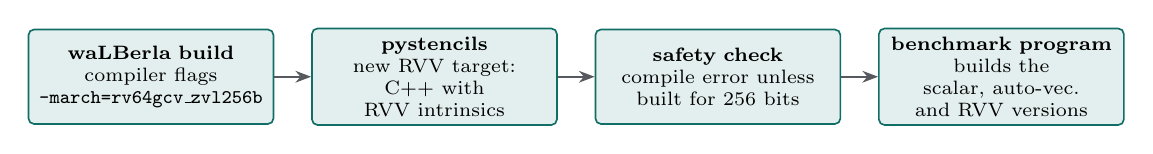
\begin{tikzpicture}[
    pc/.style={added,text width=29mm,minimum height=12mm,font=\scriptsize,align=center}]
  \def\dx{3.6}
  \node[pc] (a1) at (0,0)     {\textbf{waLBerla build}\\compiler flags\\\code{-march=rv64gcv\_zvl256b}};
  \node[pc] (a2) at (\dx,0)   {\textbf{pystencils}\\new RVV target:\\C++ with RVV intrinsics};
  \node[pc] (a3) at (2*\dx,0) {\textbf{safety check}\\compile error unless\\built for 256 bits};
  \node[pc] (a4) at (3*\dx,0) {\textbf{benchmark program}\\builds the scalar, auto-vec.\\and RVV versions};
  \foreach \u/\v in {a1/a2,a2/a3,a3/a4} \draw[arr] (\u) -- (\v);
\end{tikzpicture}


  \vspace{5mm}
  {\footnotesize\renewcommand{\arraystretch}{1.15}
  \begin{tabular}{@{}lll@{}}
    \toprule
    \textbf{build} & \textbf{kernel} & \textbf{compiler flags}\\
    \midrule
    plain scalar & plain C++ & \code{-march=rv64gc}: no vector instructions\\
    auto-vectorized & plain C++ & \code{-march=rv64gcv\_zvl256b}: GCC may vectorize\\
    best scalar & plain C++ with \term{CSE} and the in-place update & \code{-march=rv64gc}\\
    \textbf{RVV} & \textbf{RVV intrinsics from pystencils} & \code{-march=rv64gcv\_zvl256b}\\
    \bottomrule
  \end{tabular}\par}

  \vspace{2mm}
  {\scriptsize\color{psgray}Speedup: MLUP/s divided by that of the plain scalar build, same
  session. CSE: each repeated part of the formulas is computed once.\par}
  \takeaway{Users change nothing: ``optimise for this machine'' now gives RVV code, as it gives AVX
    code on x86.}
\end{frame}

% =============================================================================
\section{Part 2: make it fast}

\begin{frame}{The real limit: too many data streams}
  \begin{columns}[T,onlytextwidth]
    \column{0.52\textwidth}
    \centering% Slide 9: cost of concurrent read streams on one X60 core (r03, from board-logs/p2-stream-sweep.txt
% and p2-prefetch.txt): f32 vector loads, 4 MB per stream, huge pages.
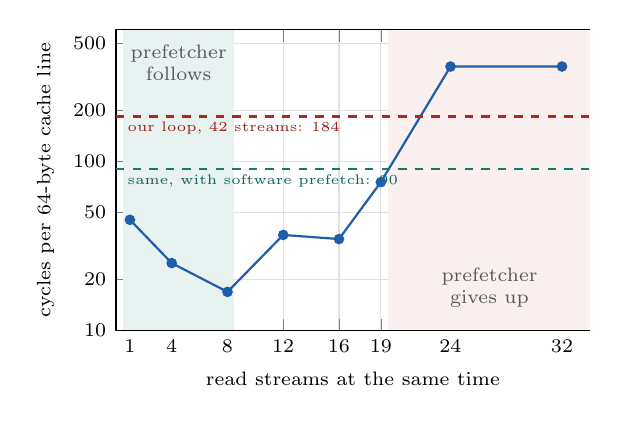
\begin{tikzpicture}
  \begin{semilogyaxis}[
      width=7.6cm, height=5.4cm,
      xlabel={read streams at the same time},
      ylabel={cycles per 64-byte cache line},
      xmin=0, xmax=34, ymin=10, ymax=600,
      xtick={1,4,8,12,16,19,24,32},
      ytick={10,20,50,100,200,500},
      yticklabels={10,20,50,100,200,500},
      grid=major, grid style={psgray!20},
      tick label style={font=\scriptsize}, label style={font=\scriptsize},
      every axis plot/.append style={thick},
    ]
    \fill[psteal!10] (axis cs:0.5,10) rectangle (axis cs:8.5,600);
    \node[lbl,anchor=north] at (axis cs:4.5,560) {prefetcher\\follows};
    \fill[psred!7] (axis cs:19.5,10) rectangle (axis cs:34,600);
    \node[lbl,anchor=south] at (axis cs:26.8,12) {prefetcher\\gives up};
    \addplot[color=psblue,mark=*,mark size=1.5pt] coordinates {
      (1,45.1) (4,25.0) (8,16.9) (12,36.7) (16,34.7) (19,75.3) (24,363.6) (32,363.7)};
    \draw[psred,thick,dashed] (axis cs:0,184.3) -- (axis cs:34,184.3);
    \node[font=\tiny,anchor=north west,text=psred!85!black,inner sep=1pt] at (axis cs:0.6,178)
      {our loop, 42 streams: 184};
    \draw[psteal,thick,dashed] (axis cs:0,90.4) -- (axis cs:34,90.4);
    \node[font=\tiny,anchor=north west,text=psteal!80!black,inner sep=1pt] at (axis cs:0.6,87)
      {same, with software prefetch: 90};
  \end{semilogyaxis}
\end{tikzpicture}

    \column{0.45\textwidth}
    \vspace{4mm}
    \begin{itemize}\small
      \item \term{Stream}: one array read or written in order. Our loop has 42 (19 read, 19
            written, 4 outputs). Fewer: update in place (23), drop the outputs (19), split the loop.
      \item Plot: a test loop reading $N$ arrays. Up to 8 the \term{hardware prefetcher} keeps up;
            past 20 it gives up, and each cache line waits for memory.
    \end{itemize}
  \end{columns}
  \takeaway{The core waits, it does not compute: 92\,\% of the time, at only 0.4\,GB/s.}
\end{frame}

% -----------------------------------------------------------------------------
%  Gains: one-session run (docs/notes3/board-logs/presentation3/): prefetch = explicit_cse ->
%  explicit_cse_pf, in place = explicit_cse_pf -> explicit_cse_aa_pf, split = explicit_cse_aa_pf ->
%  explicit_cse_aa_split. Instruction choice: kernel lab, f32 in place, 234 -> 192 cycles per cell.
%  Row addresses: r03 run C against run B. Halo copy: e2e-halo against e2e-cg. No output:
%  e2e-final-last against e2e-final. Dropped ones: report r03.
\begin{frame}{All the optimizations we tried}
  \vspace{1mm}
  {\footnotesize\renewcommand{\arraystretch}{1.12}
  \newcommand{\kept}{\textcolor{psteal!85!black}{\textbf{kept}}}
  \newcommand{\dropped}{\textcolor{psred!85!black}{dropped}}
  \newcommand{\optional}{\textcolor{psorange!90!black}{option}}
  \newcommand{\open}{\textcolor{psorange!90!black}{open}}
  \begin{tabularx}{\textwidth}{@{}l>{\raggedright\arraybackslash}Xll@{}}
    \toprule
    \textbf{optimization} & \textbf{what it does} & \textbf{gain, f32 / f64} & \textbf{result}\\
    \midrule
    software prefetch & load each array 128 bytes ahead (\term{Zicbop}) & \sx{2.04} / \sx{2.13} & \kept\\
    in-place update & AB: read A, write B. AA: read and write A & \sx{1.45} / \sx{1.57} & \kept\\
    instruction choice & scalar operands, fused multiply-add & kernel \sx{1.22} (f32) & \kept\\
    row addresses once per row & compute row start addresses once & +2.5 / +2.2\,\% & \kept\\
    halo copy per direction & copy only the values that cross a border & +2 to 6\,\% & \kept\\
    no density, velocity output & write them only in the last step & +15 / +22\,\% & \optional\\
    split loop & passes over a few directions at a time & $-$19 / +11\,\% & \open\\
    \midrule
    2 or 4 registers per instruction & longer vectors per instruction & slower & \dropped\\
    arrays aligned to 64 bytes & start each array on a cache line & 11 to 29\,\% slower & \dropped\\
    zeroing cache lines before writes & skip reading lines that are overwritten & no gain & \dropped\\
    Clang with X60 tuning & the other compiler, tuned for this core & slower than GCC & \dropped\\
    \bottomrule
  \end{tabularx}\par}

  \vspace{1.5mm}
  {\scriptsize\color{psgray}Whole program on one core, each against the same build without it.\par}
\end{frame}

% -----------------------------------------------------------------------------
\begin{frame}{Update in place: the AA pattern}
  \vspace{1mm}
  {\small The name: the usual way reads array A and writes array B (AB). This way only uses A (AA).\par}
  \begin{columns}[T,onlytextwidth]
    \column{0.4\textwidth}
    {\small\bfseries AB pattern (before)\par}
    \vspace{3mm}
    \centering% The usual "AB" scheme: two arrays, A and B. Each step reads one and writes the other, then
% they swap roles. Shown next to the AA pattern (aa-pattern.tex), which uses only array A.
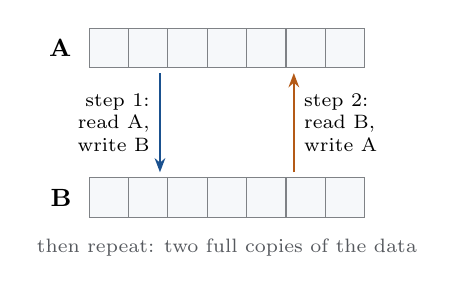
\begin{tikzpicture}[
    cell/.style={draw=psgray!80,fill=codebg,minimum width=5mm,minimum height=5mm,inner sep=0pt},
    st/.style={-{Stealth[length=1.8mm]},thick}]
  \foreach \k in {0,...,6} {
    \node[cell] at (\k*0.5+0.25,0) {};
    \node[cell] at (\k*0.5+0.25,-1.9) {};
  }
  \node[font=\small\bfseries,anchor=east] at (-0.1,0) {A};
  \node[font=\small\bfseries,anchor=east] at (-0.1,-1.9) {B};
  \draw[st,psblue!85!black] (0.9,-0.32) -- node[left,font=\scriptsize,align=right,text=black] {step 1:\\read A,\\write B} (0.9,-1.58);
  \draw[st,psorange!90!black] (2.6,-1.58) -- node[right,font=\scriptsize,align=left,text=black] {step 2:\\read B,\\write A} (2.6,-0.32);
  \node[lbl,anchor=north] at (1.75,-2.3) {then repeat: two full copies of the data};
\end{tikzpicture}


    \vspace{1mm}
    {\small\textbf{42 streams}, 260 bytes per cell\par}
    \column{0.56\textwidth}
    {\small\bfseries AA pattern: one array, two kinds of step\par}
    \vspace{1mm}
    \centering% Slide 12: the AA pattern for one pair of directions, east (E) and west (W), seen from cell x
% (as in lbmpy's AA accessors). Even step: read both slots of x, write each value into the
% other's slot of x. Odd step: read from the neighbours' slots, write to the neighbours' slots.
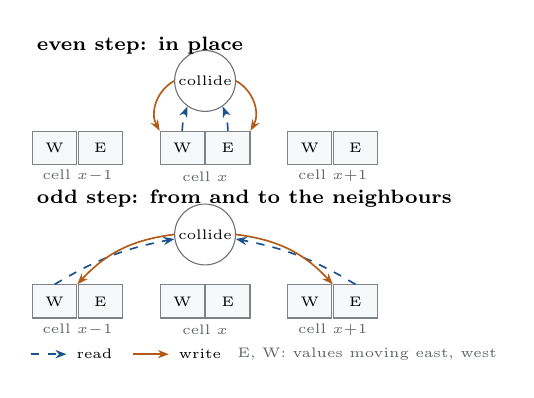
\begin{tikzpicture}[
    slot/.style={draw=psgray!80,fill=codebg,minimum width=5.6mm,minimum height=4.2mm,inner sep=0pt,font=\tiny},
    coll/.style={circle,draw=psgray!90,fill=white,inner sep=1pt,font=\tiny},
    rd/.style={-{Stealth[length=1.4mm]},semithick,draw=psblue!85!black,dashed},
    wr/.style={-{Stealth[length=1.4mm]},semithick,draw=psorange!90!black}]
  \foreach \p/\py/\ttl in {e/0/{even step: in place}, o/-1.95/{odd step: from and to the neighbours}} {
    \foreach \c/\lab in {0/$x{-}1$, 1/$x$, 2/$x{+}1$} {
      \node[slot] (\p W\c) at (\c*1.62+0.3,\py) {W};
      \node[slot] (\p E\c) at (\c*1.62+0.88,\py) {E};
      \node[font=\tiny,text=psgray] at (\c*1.62+0.59,\py-0.36) {cell \lab};
    }
    \node[coll] (\p col) at (2.21,\py+0.85) {collide};
    \node[font=\scriptsize\bfseries,anchor=west] at (-0.05,\py+1.3) {\ttl};
  }
  \draw[rd] (eE1.north) to[bend right=10] (ecol);
  \draw[rd] (eW1.north) to[bend left=10] (ecol);
  \draw[wr] (ecol.west) to[bend right=45] (eW1.north west);
  \draw[wr] (ecol.east) to[bend left=45] (eE1.north east);
  \draw[rd] (oW0.north) to[bend left=10] (ocol);
  \draw[rd] (oE2.north) to[bend right=10] (ocol);
  \draw[wr] (ocol.east) to[bend left=20] (oE2.north west);
  \draw[wr] (ocol.west) to[bend right=20] (oW0.north east);
  \draw[rd] (0,-2.62) -- ++(0.45,0) node[right,font=\tiny,text=black] {read};
  \draw[wr] (1.3,-2.62) -- ++(0.45,0) node[right,font=\tiny,text=black] {write};
  \node[font=\tiny,text=psgray,anchor=west] at (2.5,-2.62) {E, W: values moving east, west};
\end{tikzpicture}


    \vspace{1mm}
    {\small\textbf{23 streams}, 184 bytes per cell\par}
  \end{columns}
  \takeaway{New sweepgen kernels and halo exchange. Whole program, with prefetch: \sx{1.45}
    (f32), \sx{1.57} (f64).}
\end{frame}

% =============================================================================
\section{Results and limits}

\begin{frame}{Results: the whole program on one core}
  \vspace{1mm}
  \centering% Slide "Results": whole-program speedup over the plain scalar build, GCC 14, 64^3 cells, one
% core, best of 3 runs of 200 steps. All bars from one session (board 2026-11-14,
% scripts/presentation3/all.sh, logs docs/notes3/board-logs/presentation3/
% walberla-{scalar,autovec,rvv}-{f32,f64}-1core.log). Under each group: MLUP/s, f32 / f64.
%   plain = scalar (1.417 / 1.020 MLUP/s), plain auto = autovec, best = scalar_cse_aa,
%   best auto = autovec_cse_aa (auto-vectorized bars hatched), RVV AB = explicit_cse,
%   + prefetch = explicit_cse_pf, + in place = explicit_cse_aa_pf.
%   RVV now vs best scalar: 7.268 / 2.116 = 3.44 (f32), 4.299 / 1.505 = 2.86 (f64).
% Every RVV bar already has the new instruction choice and row addresses.
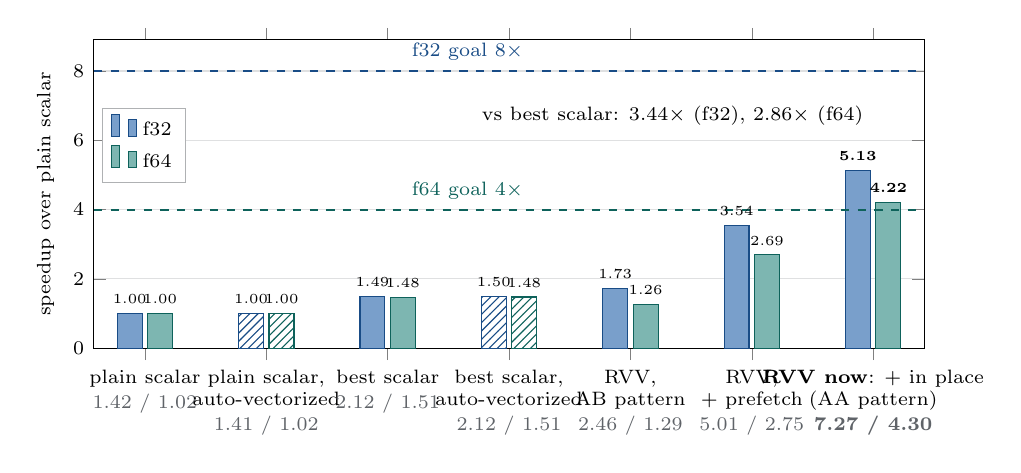
\begin{tikzpicture}
  \begin{axis}[
      ybar=2pt, bar width=9pt,
      width=\textwidth, height=5.5cm,
      ymin=0, ymax=8.9,
      ylabel={speedup over plain scalar},
      symbolic x coords={plain,plainav,best,bestav,rvv,pf,aa},
      xtick={plain,plainav,best,bestav,rvv,pf,aa},
      xticklabels={
        {plain scalar\\[1pt]\textcolor{psgray}{1.42 / 1.02}},
        {plain scalar,\\auto-vectorized\\[1pt]\textcolor{psgray}{1.41 / 1.02}},
        {best scalar\\[1pt]\textcolor{psgray}{2.12 / 1.51}},
        {best scalar,\\auto-vectorized\\[1pt]\textcolor{psgray}{2.12 / 1.51}},
        {RVV,\\AB pattern\\[1pt]\textcolor{psgray}{2.46 / 1.29}},
        {RVV,\\+ prefetch\\[1pt]\textcolor{psgray}{5.01 / 2.75}},
        {\textbf{RVV now}: + in place\\(AA pattern)\\[1pt]\textcolor{psgray}{\textbf{7.27 / 4.30}}}},
      xticklabel style={align=center,font=\scriptsize,anchor=north},
      tick label style={font=\scriptsize}, label style={font=\scriptsize},
      enlarge x limits=0.07,
      legend style={font=\scriptsize,at={(0.01,0.78)},anchor=north west,draw=psgray!50},
      nodes near coords, nodes near coords style={font=\tiny,anchor=south},
      point meta=explicit symbolic,
      ymajorgrids, grid style={psgray!20},
    ]
    \addplot[fill=psblue!60,draw=psblue!80!black,bar shift=-5.5pt] coordinates {
      (plain,1.00)[1.00] (best,1.493)[1.49] (rvv,1.734)[1.73] (pf,3.538)[3.54] (aa,5.130)[\textbf{5.13}]};
    \addplot[fill=psteal!55,draw=psteal!80!black,bar shift=5.5pt] coordinates {
      (plain,1.00)[1.00] (best,1.477)[1.48] (rvv,1.264)[1.26] (pf,2.693)[2.69] (aa,4.216)[\textbf{4.22}]};
    \addplot[pattern=north east lines,pattern color=psblue!80!black,draw=psblue!80!black,
      bar shift=-5.5pt,forget plot] coordinates {(plainav,0.997)[1.00] (bestav,1.496)[1.50]};
    \addplot[pattern=north east lines,pattern color=psteal!80!black,draw=psteal!80!black,
      bar shift=5.5pt,forget plot] coordinates {(plainav,0.999)[1.00] (bestav,1.478)[1.48]};
    \legend{f32, f64}
    \draw[psblue!80!black,dashed,thick] (axis description cs:0,8/8.9) -- (axis description cs:1,8/8.9)
      node[pos=0.45,above,font=\scriptsize] {f32 goal \sx{8}};
    \draw[psteal!80!black,dashed,thick] (axis description cs:0,4/8.9) -- (axis description cs:1,4/8.9)
      node[pos=0.45,above,font=\scriptsize] {f64 goal \sx{4}};
    \node[font=\scriptsize,anchor=south east,align=right] at (axis cs:aa,6.15)
      {vs best scalar: \sx{3.44} (f32), \sx{2.86} (f64)};
  \end{axis}
\end{tikzpicture}


  \vspace{0.5mm}
  {\scriptsize\color{psgray}Grey: MLUP/s, f32 / f64. Hatched: auto-vectorized. $64^3$ cells, 200 steps,
  best of 3 runs, one session.\par}
  \takeaway{f64 reaches its \sx{4} goal. f32 is at \sx{5.13} of the possible \sx{8}.
    Auto-vectorization gives nothing.}
\end{frame}

% -----------------------------------------------------------------------------
\begin{frame}{Several cores: the shared memory becomes the limit}
  \vspace{1mm}
  \centering% Several cores: MLUP/s of all cores together, one 64^3 block per MPI process, GCC 14, best of
% 3 runs of 200 steps. 1, 4 and 8 cores from one session (board 2026-11-14,
% scripts/presentation3/all.sh, logs docs/notes3/board-logs/presentation3/
% walberla-{scalar,autovec,rvv}-{f32,f64}-{1,4,8}core.log).
% plain scalar = scalar, best scalar = scalar_cse_aa, auto-vec. in place = autovec_cse_aa
% (hatched), RVV now = explicit_cse_aa_pf.
% Memory traffic of RVV now (184 bytes per cell in f32, 368 in f64): 4 cores 3.1 / 3.9 GB/s,
% 8 cores 4.2 / 4.0 GB/s.
% Both panels share ymax (set in the mc style) so f32 and f64 bars compare by height.
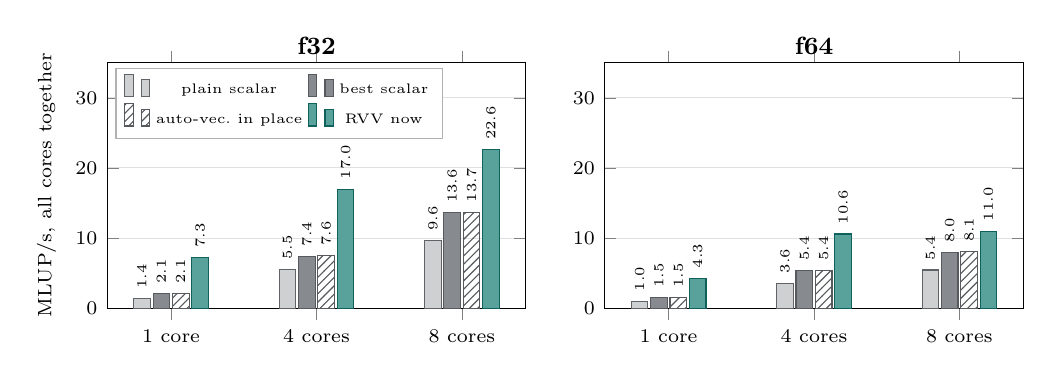
\begin{tikzpicture}
  \pgfplotsset{mc/.style={
      ybar=1pt, bar width=6pt, width=6.9cm, height=4.7cm, ymin=0, ymax=35,
      symbolic x coords={1,4,8}, xtick=data,
      xticklabels={1 core,4 cores,8 cores},
      enlarge x limits=0.22,
      tick label style={font=\scriptsize}, label style={font=\scriptsize},
      title style={font=\small\bfseries,yshift=-1.5ex},
      ymajorgrids, grid style={psgray!20},
      nodes near coords, point meta=explicit symbolic,
      nodes near coords style={font=\tiny,rotate=90,anchor=west},
    },
    pl/.style={fill=psgray!30,draw=psgray},
    bs/.style={fill=psgray!75,draw=psgray!90!black},
    av/.style={pattern=north east lines,pattern color=psgray!90!black,draw=psgray!90!black},
    rv/.style={fill=psteal!70,draw=psteal!80!black}}
  \begin{axis}[mc, name=a32, title={f32}, ylabel={MLUP/s, all cores together},
      legend style={font=\tiny,at={(0.02,0.98)},anchor=north west,draw=psgray!50},
      legend columns=2]
    \addplot[pl] coordinates {(1,1.42)[1.4] (4,5.50)[5.5] (8,9.64)[9.6]};
    \addplot[bs] coordinates {(1,2.12)[2.1] (4,7.43)[7.4] (8,13.63)[13.6]};
    \addplot[av] coordinates {(1,2.12)[2.1] (4,7.56)[7.6] (8,13.70)[13.7]};
    \addplot[rv] coordinates {(1,7.27)[7.3] (4,16.98)[17.0] (8,22.61)[22.6]};
    \legend{plain scalar, best scalar, auto-vec.\ in place, RVV now}
  \end{axis}
  \begin{axis}[mc, at={(a32.east)}, anchor=west, xshift=1.0cm, title={f64}]
    \addplot[pl] coordinates {(1,1.02)[1.0] (4,3.59)[3.6] (8,5.45)[5.4]};
    \addplot[bs] coordinates {(1,1.51)[1.5] (4,5.39)[5.4] (8,7.98)[8.0]};
    \addplot[av] coordinates {(1,1.51)[1.5] (4,5.42)[5.4] (8,8.05)[8.1]};
    \addplot[rv] coordinates {(1,4.30)[4.3] (4,10.59)[10.6] (8,10.99)[11.0]};
  \end{axis}
\end{tikzpicture}


  \vspace{1mm}
  \raggedright
  \begin{itemize}\small
    \item Each core runs one process with its own $64^3$ block.
    \item From 4 to 8 cores RVV gains 33\,\% (f32) and 4\,\% (f64): all cores together move
          at most about 4\,GB/s.
  \end{itemize}
  {\scriptsize\color{psgray}One session, best of 3 runs of 200 steps. Hatched: the best scalar
  build, auto-vectorized.\par}
  \takeaway{8 cores: RVV is \sx{2.35} (f32) and \sx{2.02} (f64) the plain scalar build, \sx{1.66}
    and \sx{1.38} the best scalar build.}
\end{frame}

% -----------------------------------------------------------------------------
%  All builds, one session: docs/notes3/board-logs/presentation3/ (board 2026-11-14), table at
%  the end of walberla-presentation.log. scripts/presentation3/all.sh reruns it.
\begin{frame}{Numbers: every build in one session}
  \vspace{1mm}
  \centering
  {\footnotesize\renewcommand{\arraystretch}{1.05}
  \begin{tabular}{@{}lrrrrrr@{}}
    \toprule
    & \multicolumn{2}{c}{\textbf{1 core}} & \multicolumn{2}{c}{\textbf{4 cores}}
      & \multicolumn{2}{c}{\textbf{8 cores}}\\
    \cmidrule(lr){2-3}\cmidrule(lr){4-5}\cmidrule(l){6-7}
    MLUP/s, all cores together & f32 & f64 & f32 & f64 & f32 & f64\\
    \midrule
    plain scalar & 1.42 & 1.02 & 5.50 & 3.59 & 9.64 & 5.45\\
    scalar, CSE & 1.59 & 1.08 & 5.83 & 3.74 & 9.90 & 5.60\\
    scalar, CSE, in place (best scalar) & 2.12 & 1.51 & 7.43 & 5.39 & 13.63 & 7.98\\
    \midrule
    auto-vectorized & 1.41 & 1.02 & 5.51 & 3.57 & 9.64 & 5.44\\
    auto-vectorized, CSE & 1.59 & 1.08 & 5.78 & 3.74 & 9.99 & 5.60\\
    auto-vectorized, CSE, in place & 2.12 & 1.51 & 7.56 & 5.42 & 13.70 & 8.05\\
    \midrule
    RVV, CSE & 2.46 & 1.29 & 7.98 & 4.17 & 12.02 & 5.85\\
    RVV, CSE, prefetch & 5.01 & 2.75 & 12.46 & 6.90 & 15.72 & 7.57\\
    RVV, CSE, in place & 3.03 & 1.52 & 9.34 & 5.24 & 15.45 & 7.75\\
    \textbf{RVV, CSE, in place, prefetch (now)} & \textbf{7.27} & \textbf{4.30} & \textbf{16.98}
      & \textbf{10.59} & \textbf{22.61} & \textbf{10.99}\\
    RVV, CSE, in place, prefetch, split loop & 5.91 & 4.77 & 17.77 & 10.83 & 22.44 & 10.99\\
    \bottomrule
  \end{tabular}\par}

  \vspace{3mm}
  \raggedright
  {\scriptsize\color{psgray}
  Whole program, one process per core with its own $64^3$ block, GCC~14, best of 3 runs of 200
  time steps. The f64 checksums are identical across all builds, the f32 ones agree to
  $2\cdot 10^{-5}$. One script reruns all of it in about 4 hours:
  \code{scripts/presentation3/all.sh}.\par}
\end{frame}

% -----------------------------------------------------------------------------
\begin{frame}{Where the code and the details are}
  \vspace{1mm}
  \small
  \begin{tabularx}{\textwidth}{@{}l l X@{}}
    \toprule
    Repository & Branch, commit & Contents\\
    \midrule
    \href{https://github.com/salehjg/mirrored-pystencil2/tree/rvv-support}{\code{mirrored-pystencil2}}
      & \code{rvv-support}, \code{a81dc547} & pystencils: RVV target, prefetch, instruction choice\\
    \href{https://github.com/salehjg/mirrored-walberla/tree/rvv-support}{\code{mirrored-walberla}}
      & \code{rvv-support}, \code{efa2b70c} & waLBerla: flags, in-place update, benchmark\\
    \href{https://github.com/salehjg/my-e4-ws}{\code{my-e4-ws}} & \code{main}, \code{c443bf4}
      & workspace: both forks, scripts, raw logs\\
    \bottomrule
  \end{tabularx}

  \vspace{4mm}
  Written reports in the workspace, \code{docs/manual/} (\code{./build.sh}):
  \begin{itemize}\small
    \item Report 2: RISC-V vector support in waLBerla (part 1 of this talk, about 60 pages).
    \item Report 3: toward \sx{8} with RVV on the SpacemiT K1 (part 2, about 45 pages), with
          the log file behind every number.
  \end{itemize}
  \vfill
  \centering{\Huge\bfseries\color{psred}Thank you\par}
  \vspace{2mm}
\end{frame}

% =============================================================================
\appendix
\section{Backup}

\begin{frame}{Glossary (1/2)}
  \begin{columns}[T,onlytextwidth]
    \column{0.49\textwidth}
    \scriptsize
    \begin{description}\setlength{\itemsep}{1.5pt}
      \item[AA pattern] in-place update: one array (A) is read and written; even and odd steps alternate.
      \item[AB pattern] the usual update: read array A, write array B, then swap.
      \item[Auto-vectorization] the compiler turns a plain loop into vector code by itself.
      \item[Best scalar build] no vector instructions, but with the other improvements (CSE, AA pattern).
      \item[Block] a box of cells; waLBerla cuts the domain into blocks, here one per process.
      \item[Build time] when the program is compiled; here code generation happens too.
      \item[Cache line] the unit the memory system moves: 64 bytes on the X60.
      \item[CSE] common sub-expression elimination: compute each repeated part of a formula once.
      \item[D3Q19] the LBM model used: 3 dimensions, 19 directions per cell.
      \item[f32, f64] single (32-bit) and double (64-bit) precision floating point.
    \end{description}
    \column{0.49\textwidth}
    \scriptsize
    \begin{description}\setlength{\itemsep}{1.5pt}
      \item[FMA] fused multiply-add: $a \cdot b + c$ in one instruction, rounded once.
      \item[Generator script] a Python file per program that says which kernels to generate.
      \item[Ghost layer] a one-cell copy of the neighbour block's border around each block.
      \item[Halo exchange] refreshing the ghost layers after each time step.
      \item[Hardware prefetcher] part of the cache that spots regular access patterns and loads data early.
      \item[Intrinsic] a C/C++ function that the compiler turns into one machine instruction.
      \item[K1, X60] the SpacemiT chip on the board, and its core type.
      \item[Kernel] the generated loop that updates all cells once.
      \item[Kernel lab] a small program that times one kernel alone, without waLBerla.
    \end{description}
  \end{columns}
\end{frame}

\begin{frame}{Glossary (2/2)}
  \begin{columns}[T,onlytextwidth]
    \column{0.49\textwidth}
    \scriptsize
    \begin{description}\setlength{\itemsep}{1.5pt}
      \item[Lane] one number's slot in a vector register: 8 for f32, 4 for f64.
      \item[LBM] lattice Boltzmann method: fluid simulation on a grid of cells.
      \item[lbmpy] Python package that derives the LBM formulas for one cell.
      \item[MLUP/s] million cell updates per second.
      \item[MPI] the standard library for messages between processes, also between computers.
      \item[Plain scalar build] the same program compiled without any vector instructions.
      \item[pystencils] Python package that turns formulas into a C++ loop over all cells.
      \item[QEMU] an emulator that runs RISC-V programs on an x86 computer.
      \item[RISC-V] an open instruction set architecture.
    \end{description}
    \column{0.49\textwidth}
    \scriptsize
    \begin{description}\setlength{\itemsep}{1.5pt}
      \item[Run time] when the compiled program runs.
      \item[RVV] the RISC-V vector extension.
      \item[Software prefetch] an instruction that asks the cache to load data that will be needed soon.
      \item[Spill] saving a register to memory and loading it back, for lack of registers.
      \item[SRT] single relaxation time: the simplest LBM collision model.
      \item[Stream] a walk through one array in order.
      \item[sweepgen] part of waLBerla: wraps generated kernels into C++ classes.
      \item[.vf form] an RVV instruction form with one vector and one scalar operand.
      \item[waLBerla] open-source C++ framework for fluid simulations.
      \item[Zicbop] the RISC-V extension with the prefetch instructions.
    \end{description}
  \end{columns}
\end{frame}

% -----------------------------------------------------------------------------
\begin{frame}{Numbers: one step at a time}
  \vspace{1mm}
  \centering
  {\small
  \begin{tabular}{@{}lrrrr@{}}
    \toprule
    & \multicolumn{2}{c}{\textbf{f32}} & \multicolumn{2}{c}{\textbf{f64}}\\
    \cmidrule(lr){2-3}\cmidrule(l){4-5}
    Step & MLUP/s & vs plain & MLUP/s & vs plain\\
    \midrule
    plain scalar build & 1.40 & \sx{1.00} & 0.95 & \sx{1.00}\\
    best scalar build (CSE, in-place update) & 2.05 & \sx{1.46} & 1.44 & \sx{1.51}\\
    RVV code at the start of part 2 & 2.40 & \sx{1.72} & 1.21 & \sx{1.26}\\
    + software prefetch & 4.70 & \sx{3.36} & 2.37 & \sx{2.48}\\
    + in-place update and new instruction choice & 7.08 & \sx{5.06} & 3.95 & \sx{4.14}\\
    + row addresses once per row (second session) & 7.25 & \sx{5.24} & 4.04 & \sx{4.23}\\
    \bottomrule
  \end{tabular}\par}

  \vspace{3mm}
  \raggedright
  {\scriptsize\color{psgray}
  Whole program (kernel, halo exchange, time loop), $64^3$ cells, one core, GCC~14, best of 3
  runs of 200 time steps. Rows 1 to 5 are from one session; the last row is from a second
  session and is compared with that session's own scalar build (1.38 and 0.95\,MLUP/s). The
  part 1 measurement (\sx{1.73}, \sx{1.31}) is an earlier session. Lab: hand-written split loop
  10.83\,MLUP/s (cycle average, Clang with X60 tuning) against 1.40 for the plain scalar build:
  \sx{7.7}. The results slides use a later session with every build (table at the end of the talk).\par}
\end{frame}

% -----------------------------------------------------------------------------
\begin{frame}{How we know the results are still correct}
  \vspace{1mm}
  \centering
  {\footnotesize
  \begin{tabular}{@{}l>{\centering\arraybackslash}p{2.6cm}>{\centering\arraybackslash}p{2.2cm}>{\centering\arraybackslash}p{1.6cm}@{}}
    \toprule
    Change & waLBerla tests on x86, 1, 2, 4 processes & same checksum, whole program
      & emulator (QEMU)\\
    \midrule
    software prefetch & \no & \yes & \no\\
    in-place update, halo exchange & \yes & \yes & \yes\\
    instruction choice & \no & \yes & \yes\\
    row addresses & \no & \yes & \yes\\
    \bottomrule
  \end{tabular}\par}

  \vspace{4mm}
  \raggedright
  \begin{itemize}\small
    \item 24 of 24 waLBerla tests pass on x86. In f64 every build gives the same checksum, bit
          for bit, on 1, 4 and 8 cores.
    \item Tests broken on purpose fail, as they should.
    \item Found and fixed: the original benchmark's start-up gave results that depended on
          the number of blocks.
  \end{itemize}
\end{frame}

% -----------------------------------------------------------------------------
\begin{frame}{Where each change lives}
  \centering{\brmarkerstrue\resizebox{0.88\textwidth}{!}{% From source to a running simulation (report r02, chapter "Code Generation" and its figure
% build-flow.tex). CMake configures; during "make", CMake runs the Python generator scripts
% (sweepgen sets jit = no_jit: generate only), then compiles the generated C++ together with
% the hand-written waLBerla core. The executable runs without Python. Everything ran on the
% board. Violet = generated code. Each column is one step; the small arrows between the
% headers carry the results from step to step (no wires across columns).
%
% With \brmarkerstrue (slide "Where each change lives") numbered markers show what we changed:
% blue = part 1, teal = part 2 (10 to 12: the last three changes, see the open-work slide).
% The markers sit on the nodes a2, g0, g2, g3, i1, i2 and cc.
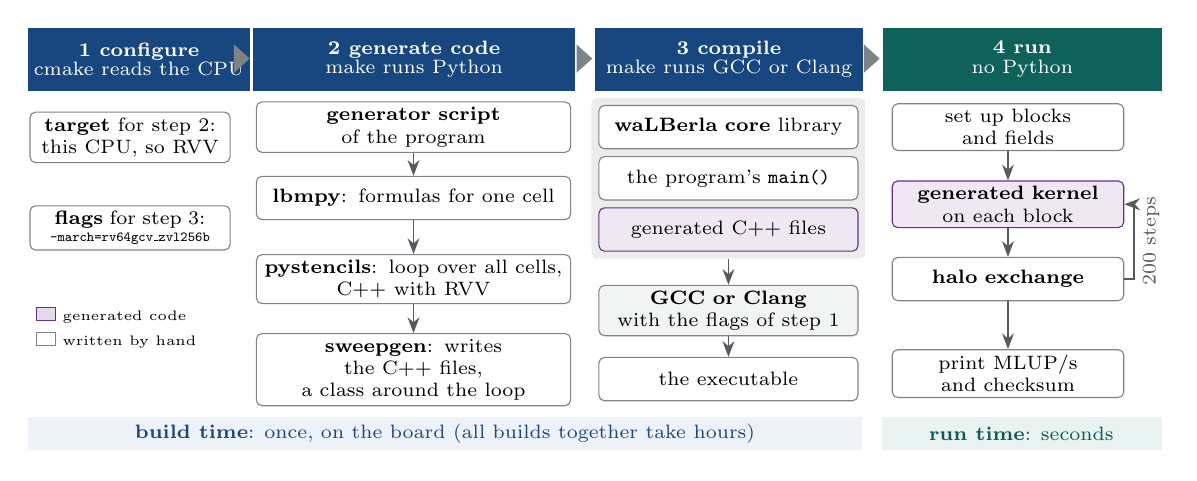
\begin{tikzpicture}[
    hdr/.style={font=\scriptsize\bfseries,text=white,align=center,inner sep=2pt,
      minimum height=8mm,anchor=north west},
    b/.style={box,font=\scriptsize,minimum height=5.5mm,inner sep=2pt,
      execute at begin node={\hyphenpenalty=10000\exhyphenpenalty=10000}},
    gen/.style={b,fill=psviolet!12,draw=psviolet!80!black},
    hdrarr/.style={fill=psgray!80},
    mk/.style={circle,text=white,font=\tiny\bfseries,inner sep=0pt,minimum size=3.7mm}]
  \ifbrmarkers\tikzset{mkl/.style={align=left}}\else\tikzset{mkl/.style={}}\fi
  % ---- column headers, with arrows from step to step --------------------------------
  \node[hdr,fill=psblue!75!black,minimum width=2.6cm] at (0,0)
    {1 configure\\[-1pt]{\mdseries cmake reads the CPU}};
  \node[hdr,fill=psblue!75!black,minimum width=4.1cm] at (2.85,0)
    {2 generate code\\[-1pt]{\mdseries make runs Python}};
  \node[hdr,fill=psblue!75!black,minimum width=3.4cm] at (7.2,0)
    {3 compile\\[-1pt]{\mdseries make runs GCC or Clang}};
  \node[hdr,fill=psteal!80!black,minimum width=3.55cm] at (10.85,0)
    {4 run\\[-1pt]{\mdseries no Python}};
  \foreach \x in {2.62,6.97,10.62}
    \fill[hdrarr] (\x,-0.22) -- ++(0.2,-0.18) -- ++(-0.2,-0.18) -- cycle;

  % ---- 1 configure: two settings for the later steps --------------------------------
  \node[b,text width=2.4cm] (a3) at (1.3,-1.4) {\textbf{target} for step 2:\\this CPU, so RVV};
  \node[b,text width=2.4cm,font=\tiny] (a2) at (1.3,-2.55)
    {{\scriptsize\textbf{flags} for step 3:}\\\code{-march=rv64gcv\_zvl256b}};
  \node[anchor=north west,font=\tiny,align=left,inner sep=0pt] at (0.1,-3.55)
    {\tikz\fill[psviolet!20,draw=psviolet!80!black] (0,0) rectangle (2.4mm,1.6mm);\ generated code\\[3pt]
     \tikz\draw[psgray!80] (0,0) rectangle (2.4mm,1.6mm);\ written by hand};

  % ---- 2 generate: the Python tool chain ---------------------------------------------
  \node[b,text width=3.85cm] (g0) at (4.9,-1.27) {\textbf{generator script} of the program};
  \node[b,text width=3.85cm] (g1) at (4.9,-2.17) {\textbf{lbmpy}: formulas for one cell};
  \node[b,text width=3.85cm] (g2) at (4.9,-3.2) {\textbf{pystencils}: loop over all cells,\\C++ with RVV};
  \node[b,text width=3.85cm] (g3) at (4.9,-4.35) {\textbf{sweepgen}: writes the C++ files,\\a class around the loop};
  \foreach \u/\v in {g0/g1,g1/g2,g2/g3} \draw[arr] (\u) -- (\v);

  % ---- 3 compile: hand-written and generated C++ together ----------------------------
  \node[b,mkl,text width=3.15cm] (i1) at (8.9,-1.27) {\textbf{waLBerla core} library};
  \node[b,mkl,text width=3.15cm] (i2) at (8.9,-1.92) {the program's \code{main()}};
  \node[gen,text width=3.15cm] (i0) at (8.9,-2.57) {generated C++ files};
  \begin{scope}[on background layer]
    \node[fill=psgray!12,rounded corners=2pt,inner sep=2.5pt,fit=(i1)(i2)(i0)] (src) {};
  \end{scope}
  \node[b,text width=3.15cm,fill=psgray!8] (cc) at (8.9,-3.6) {\textbf{GCC or Clang}\\with the flags of step 1};
  \node[b,text width=3.15cm] (exe) at (8.9,-4.47) {the executable};
  \draw[arr] (src) -- (cc);
  \draw[arr] (cc) -- (exe);

  % ---- 4 run: set up, then the time loop ---------------------------------------------
  \node[b,text width=2.8cm] (r0) at (12.45,-1.27) {set up blocks and fields};
  \node[gen,text width=2.8cm] (r1) at (12.45,-2.25) {\textbf{generated kernel}\\on each block};
  \node[b,text width=2.8cm] (r2) at (12.45,-3.2) {\textbf{halo exchange}};
  \node[b,text width=2.8cm] (r3) at (12.45,-4.4) {print MLUP/s and checksum};
  \draw[arr] (r0) -- (r1);
  \draw[arr] (r1) -- (r2);
  \draw[arr] (r2.east) -- ++(0.12,0) |- (r1.east);
  \node[lbl,rotate=90] at (14.27,-2.72) {200 steps};
  \draw[arr] (r2) -- (r3);

  % ---- time bands ----------------------------------------------------------------------
  \fill[psblue!8] (0,-4.95) rectangle (10.6,-5.37);
  \node[font=\scriptsize,text=psblue!75!black] at (5.3,-5.16)
    {\textbf{build time}: once, on the board (all builds together take hours)};
  \fill[psteal!10] (10.85,-4.95) rectangle (14.4,-5.37);
  \node[font=\scriptsize,text=psteal!75!black] at (12.62,-5.16) {\textbf{run time}: seconds};

  % ---- markers: what we changed ------------------------------------------------------
  \ifbrmarkers
    \tikzset{mk/.append style={minimum size=3.2mm}}
    %   \brmark: on top of the box's upper border; \brmarkin: inside the box, at its right end
    \def\brmark#1#2#3#4{% node, slot (0 = rightmost), colour, number
      \node[mk,fill=#3] at ([xshift={-2.2mm-#2*3.6mm},yshift=1.3mm]#1.north east) {#4};}
    \def\brmarkin#1#2#3#4{%
      \node[mk,fill=#3] at ([xshift={-2.2mm-#2*3.6mm}]#1.east) {#4};}
    \brmark{a2}{0}{psblue}{1}   \brmark{a2}{1}{psteal}{8}
    \brmark{g0}{0}{psblue}{3}
    \brmark{g2}{0}{psblue}{2}   \brmark{g2}{1}{psteal}{5}   \brmark{g2}{2}{psteal}{12}
    \brmark{g3}{0}{psteal}{6}   \brmark{g3}{1}{psteal}{10}
    \brmarkin{i1}{0}{psteal}{11} \brmarkin{i1}{1}{psteal}{7}
    \brmarkin{i2}{0}{psteal}{9}    \brmarkin{i2}{1}{psblue}{3}
    \brmark{cc}{0}{psblue}{4}
  \fi
\end{tikzpicture}
}}

  \vspace{1.5mm}
  {\scriptsize\renewcommand{\arraystretch}{0.95}
  \begin{tabular}{@{}lll@{}}
    \tagdot{psblue}\ \textbf{part 1: make it work} & \tagdot{psteal}\ \textbf{part 2: make it fast}
      & \tagdot{psteal}\ \textbf{part 2: the last three changes}\\
    1 RISC-V compiler flags & 5 prefetch, instruction choice, row addresses & 10 no density and velocity output\\
    2 RVV target in pystencils & 6 in-place kernels \quad 7 their halo exchange & 11 halo copy per direction\\
    3 benchmark program \quad 4 Clang fix & 8 X60 flag for Clang \quad 9 in-place time loop & 12 split kernel\\
  \end{tabular}\par}
\end{frame}

\end{document}
